En un videojuego, la interfaz es esencial para transmitir información al jugador tanto dentro del juego para poder interactuar con dicho mundo, como en los menús para modificar elementos externos del juego tales como guardar una partida, cambiar especificaciones de la visualización del juego, etc. Por ello, en esta sección se especificará con detalle cada una de las pantallas y los menú que componen \nombrejuego. Además, se indicarán las transiciones entre ellas así como la utilidad de cada elemento de la GUI (\emph{Graphical User Interface}) o interfaz en español. Las imágenes adjuntas son bocetos que ilustran los componentes que debe contener cada pantalla, no obstante, los artistas podrán hacer cambios en la apariencia y disposición de los elementos si así lo consideran oportuno.
    
    \newpage
    \section{HUD (\emph{Heads-Up Display})}
    El HUD es el elemento de la GUI o interfaz diseñado para mostrar información al \emph{Jugador} dentro del juego. Usualmente está para indicar la vida, munición, armas y acciones a poder realizar. En el caso de las aventuras gráficas, el HUD se usaba principalmente para mostrar el inventario de objetos del que dispone el jugador y de las acciones que este puede realizar, además de algún icono para poder acceder a otros menús.
    
    En \nombrejuego al ser una aventura gráfica, su premisa es similar a la comentada en el párrafo anterior:
    
    \begin{figure}[H] 
	     \begin{center}
	         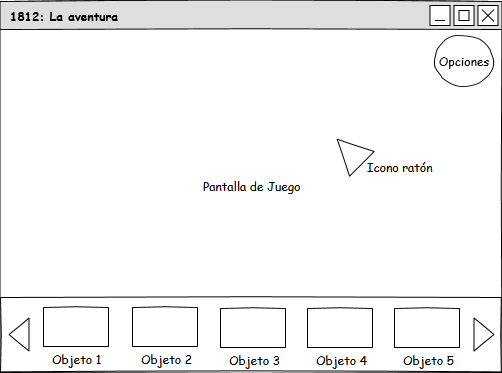
\includegraphics[scale=0.7]{dentro_del_juego.png}
	     \end{center}
	     \caption{Boceto del HUD dentro del juego}
	     \label{fig:hud-dentro-juego}
	\end{figure}
	
	Lista y descripción de todos sus componentes:
	\begin{itemize}
	\item \negrita{Botón Opciones}: al pulsarlo nos lleva a la pantalla \emph{Menú Opciones}.
	\item \negrita{Ratón del juego}: el icono del ratón dentro del juego irá cambiando según se coloque encima de un elemento con el que se pueda interaccionar.
	\item \negrita{Lista de objetos}: lista con los objetos que tiene el \emph{Jugador} en posesión hasta el momento. Para cada objeto se muestra una imagen y el nombre.
	\item \negrita{Pantalla de Juego}: Escenario 2D del juego. 
	\end{itemize}
    
    \newpage
    \label{sec:diagrama-flujo-menus}
        \section{Diagrama de flujo}
        En todo juego, los menús necesitan de una jerarquía u orden a la hora de aparecer en pantalla. Para ello, normalmente se usa un diagrama que establece de manera visual el orden y acceso a los distintos menús durante el juego. Normalmente en un juego pequeño, dónde solo hay uno o dos menús, se puede hacer innecesario. Pero en cuanto intentemos realizar un juego que necesite más de cuatro menús diferentes, se hace inviable el no esquematizar el orden de estos. No solo para el programador, sino para el jugador, pues el tener que ir buscando el menú específico de forma complicada, hará que dicho jugador se canse rápidamente del juego y consecuentemente abandonarlo. El siguiente diagrama de estados muestra las pantallas presentes a lo largo de \nombrejuego y las transiciones entre ellas.
        
        \begin{figure}[H] 
                \begin{center}
                    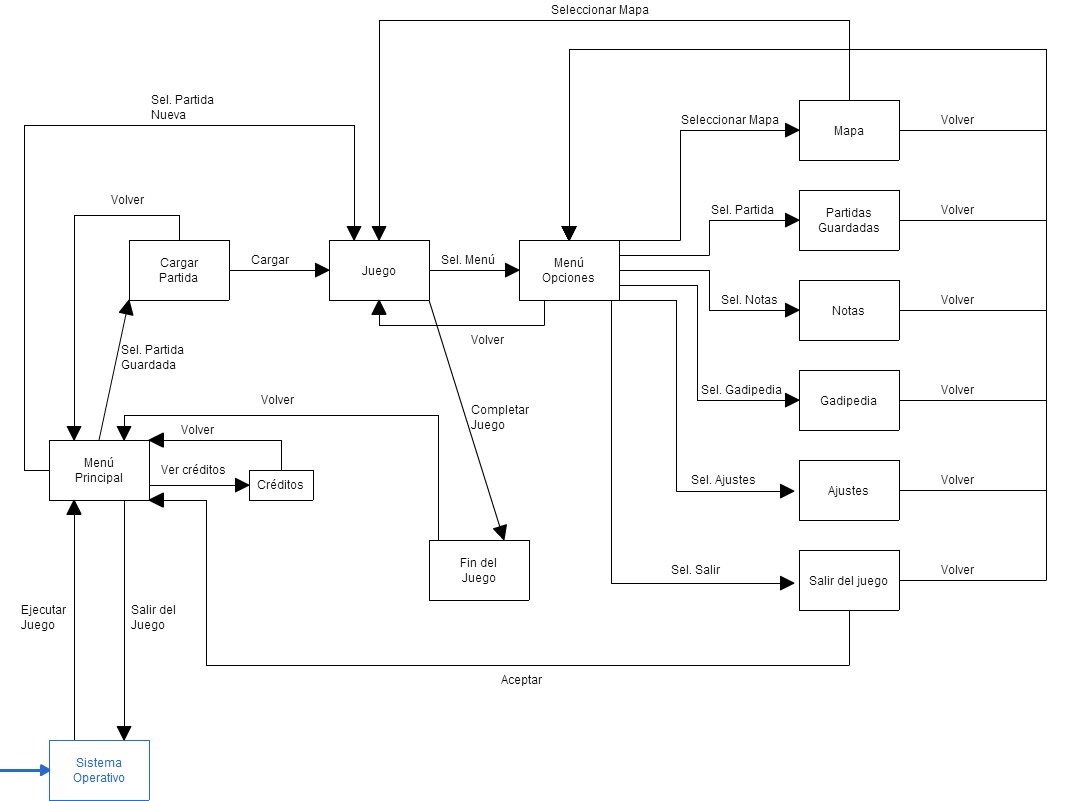
\includegraphics[scale=0.45]{diagrama_flujo_menu.png}
                \end{center}
                \caption{Diagrama de flujo de pantallas en el juego}
                \label{fig:diagrama-flujo-menu}
            \end{figure}
        
        \newpage
        \section{Descripciones de las pantallas}
        En esta sección nos centraremos en describir de manera individual todas las pantallas que hacen aparición en \nombrejuego.
        
        %\newpage
            \subsection{Menú principal}
            A continuación el boceto de la pantalla de \emph{Menú Principal} :
            
            \begin{figure}[H] 
                \begin{center}
                    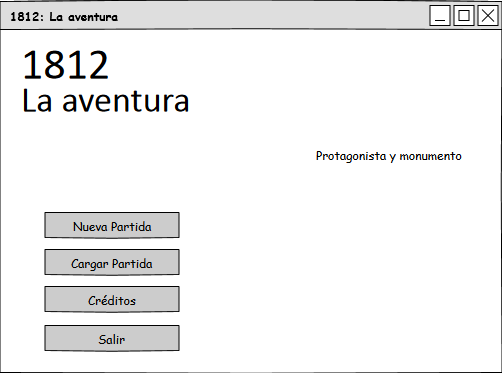
\includegraphics[scale=0.7]{men_principal.png}
                \end{center}
                \caption{Boceto del Menú Principal}
                \label{fig:menu-principal}
            \end{figure}
            
            Lista y descripción de todos sus componentes:
            \begin{itemize}
            \item \negrita{Botón Nueva Partida}: al pulsarlo lleva a la pantalla de \emph{Crear Partida}.
            \item \negrita{Botón Cargar Partida}: al pulsarlo lleva a la pantalla de \emph{Cargar Partida}.
            \item \negrita{Botón Créditos}: al pulsarlo nos lleva a la pantalla \emph{Créditos}.
            \item \negrita{Botón Salir}: al pulsarlo nos lleva de vuelta al Sistema Operativo.
            \item \negrita{Protagonista y monumento}: Una ilustración del protagonista de \nombrejuego situado en un monumento emblemático del 1812.
            \end{itemize}
            
            \newpage
            \subsection{Cargar Partida}
            A continuación el boceto de la pantalla de \emph{Cargar Partida} :
            
            \begin{figure}[H] 
                \begin{center}
                    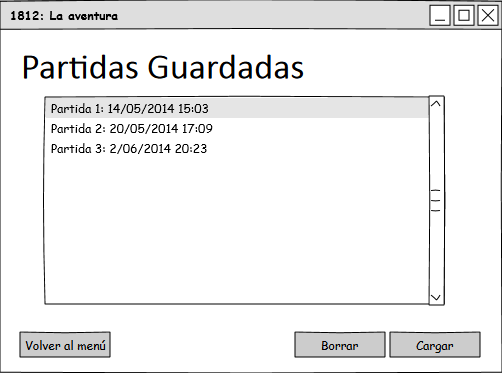
\includegraphics[scale=0.7]{cargar_partida.png}
                \end{center}
                \caption{Boceto de la pantalla de Cargar Partida}
                \label{fig:cargar-partida}
            \end{figure}
            
            Lista y descripción de todos sus componentes:
            \begin{itemize}
            \item \negrita{Lista de partidas}: lista con las partidas guardadas hasta el momento. Se muestra el día y la hora de la última actualización de esa partida.
            \item \negrita{Botón Cargar}: al pulsarlo coge la partida seleccionada y carga la pantalla de juego tal y como la dejamos.
            \item \negrita{Botón Borrar}: al pulsarlo nos dará un mensaje de aviso de si verdaderamente queremos borrar la partida, si le damos a sí nos borrará la partida, si elegimos la otra opción desaparecerá el mensaje de aviso sin realizar ningún borrado.
            \item \negrita{Botón Volver al menú}: al pulsarlo volvemos al \emph{Menú Principal}.
            \end{itemize}
            
            \newpage
            \subsection{Créditos}
            A continuación el boceto de la pantalla de \emph{Créditos} :
            
            \begin{figure}[H] 
                \begin{center}
                    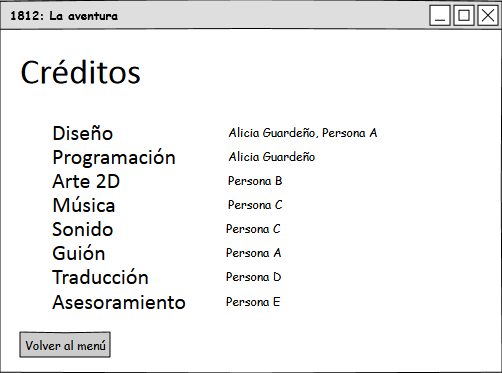
\includegraphics[scale=0.7]{crditos.png}
                \end{center}
                \caption{Boceto de la pantalla de Créditos}
                \label{fig:creditos}
            \end{figure}
            
            Lista y descripción de todos sus componentes:
            \begin{itemize}
            \item \negrita{Panel}: texto con los componentes del equipo de desarrollo.
            \item \negrita{Botón Volver al menú}: al pulsarlo volvemos al \emph{Menú Principal}.
            \end{itemize}
            
            \newpage
            \subsection{Menú Opciones}
        	A continuación el boceto de la pantalla del \emph{Menú de Opciones} :
	         
	         \begin{figure}[H] 
	             \begin{center}
	                 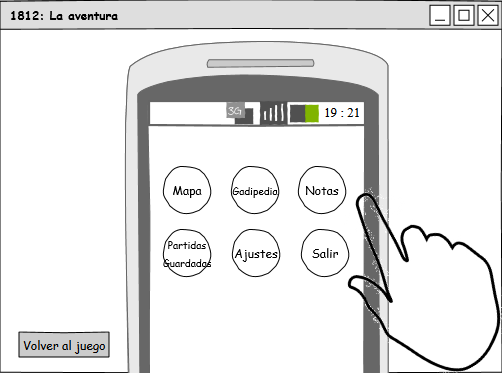
\includegraphics[scale=0.7]{men_opciones.png}
	             \end{center}
	             \caption{Boceto de la pantalla del Menú de Opciones}
	             \label{fig:menu-opciones}
	         \end{figure}
	         
	         Lista y descripción de todos sus componentes:
	         \begin{itemize}
	         \item \negrita{Icono Mapa}: al pulsarlo vamos a la pantalla \emph{Mapa}. 
	         \item \negrita{Icono Gadipedia}: al pulsarlo vamos a la pantalla \emph{Gadipedia}. 
	         \item \negrita{Icono Notas}: al pulsarlo vamos a la pantalla \emph{Notas}.
	         \item \negrita{Icono Partidas Guardadas}: al pulsarlo vamos a la pantalla \emph{Partidas Guardadas}.
	         \item \negrita{Icono Mapa}: al pulsarlo vamos a la pantalla \emph{Ajustes}.
	         \item \negrita{Icono Salir}: al pulsarlo nos saldrá un mensaje que nos preguntará si queremos salir del juego y que todo lo que no haya sido guardado se perderá, si le damos a sí volvemos al \emph{Menú Principal}, si elegimos la otra opción el mensaje desaparecerá sin realizar ninguna acción.    
	         \item \negrita{Botón Volver al menú}: al pulsarlo volvemos a la pantalla de juego.
	         \item \negrita{Imágenes \emph{smartphone} y mano}: son las imágenes del fondo de la pantalla, simulando que el personaje principal usa su \emph{smartphone} para interactuar con los diferentes menús dentro del juego.
	         \end{itemize}
        
            \newpage
            \subsection{Mapa}
            A continuación el boceto de la pantalla \emph{Mapa} :
            
            \begin{figure}[H]
            	\begin{center}
            		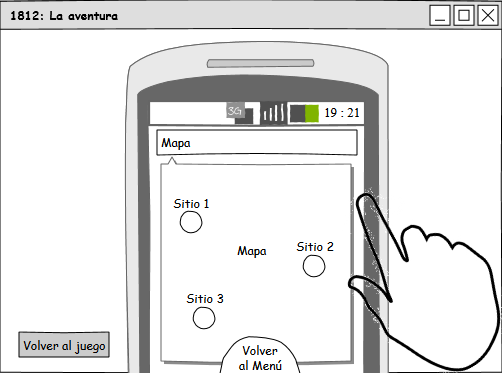
\includegraphics[scale=0.7]{mapa.png}
            	\end{center}
            	\caption{Boceto de la pantalla Mapa}
            	\label{fig:mapa}
            \end{figure}
            
            Lista y descripción de todos sus componentes:
            \begin{itemize}
            \item \negrita{Panel Mapa}: Panel con una imagen de las calles del centro de Cádiz y sus respectivos nombres.
            \item \negrita{Iconos de Sitio}: Muestran un lugar al que se puede visitar dentro del juego, irá con el nombre del lugar. Al pulsarlo saldrá un mensaje preguntándonos si queremos ir a esa localización, si le decimos que sí volveremos a la pantalla de juego pero en la ubicación especificada, si elegimos la otra opción el mensaje desaparecerá sin realizar ninguna acción.
            \item \negrita{Icono Volver al Menú}: al pulsarlo volvemos a la pantalla \emph{Menú Opciones}.
            \item \negrita{Botón Volver al juego}: al pulsarlo volvemos a la pantalla de juego.
            
            \end{itemize}
            
            \newpage
            \subsection{Partidas guardadas dentro del juego}
            A continuación el boceto de la pantalla de \emph{Partidas Guardadas} dentro del juego :
            
            \begin{figure}[H] 
                \begin{center}
                    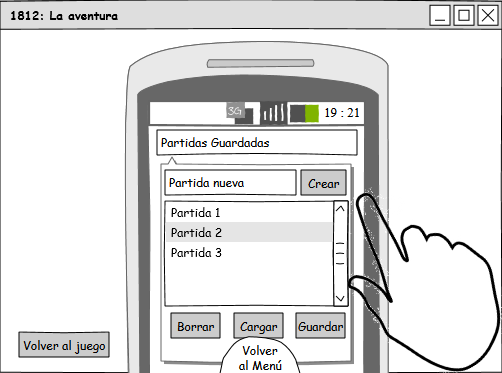
\includegraphics[scale=0.7]{cargar_partida_dentro_del_juego.png}
                \end{center}
                \caption{Boceto de la pantalla de Cargar Partida}
                \label{fig:cargar-partida-dentro-juego}
            \end{figure}
            
            Lista y descripción de todos sus componentes:
            \begin{itemize}
            \item \negrita{Crear partida nueva}: etiqueta y caja de texto para introducir el nombre de la nueva partida.
            \item \negrita{Botón Crear}: crea una nueva partida con el nombre que contiene la caja de texto. Si el perfil existe o no se ha introducido un nombre, una ventana con un mensaje aparecerá indicando el error.
            \item \negrita{Lista de partidas}: lista con las partidas guardadas hasta el momento. Se muestra el día y la hora de la última actualización de esa partida.
            \item \negrita{Icono Volver al Menú}: al pulsarlo volvemos a la pantalla \emph{Menú Opciones}.
            \item \negrita{Botón Volver al juego}: al pulsarlo volvemos a la pantalla de juego.
            \end{itemize}
            
            \newpage
            \subsection{Gadipedia}
            A continuación el boceto de la pantalla \emph{Gadipedia} :
            
            \begin{figure}[H] 
                \begin{center}
                    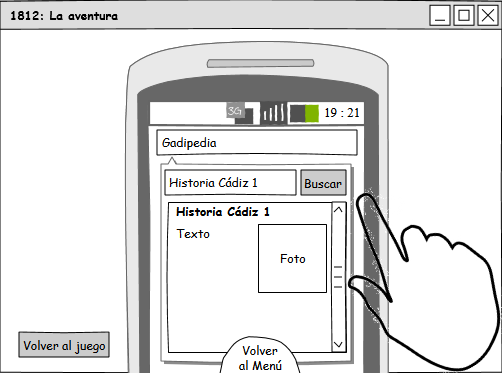
\includegraphics[scale=0.7]{gadipedia.png}
                \end{center}
                \caption{Boceto de la pantalla de Gadipedia}
                \label{fig:gadipedia}
            \end{figure}
            
            Lista y descripción de todos sus componentes:
            \begin{itemize}
            \item \negrita{Caja de texto}: caja de texto donde introducimos las palabras clave de la información que queramos saber de la historia de Cádiz de 1812.
            \item \negrita{Botón Buscar}: al pulsarlo buscará la información correspondiente a las palabras clave. Dependiendo de las palabras clave podrá pasar distintas cosas: que el buscador no encuentre ninguna información y muestre en una ventana emergente que no ha habido resultados, que las palabras clave sean ambigüas y muestre en una ventana emergente que pruebes a realizar la búsqueda con otros términos menos ambigüos, o que la búsqueda haya sido con éxito y las mostrará en el bloque de texto debajo del cuadro de búsqueda.
            \item \negrita{Bloque de texto e información}: bloque de texto informativo sobre un aspecto específico del Cádiz de 1812, podrá incluir fotos en un lado.
            \item \negrita{Icono Volver al Menú}: al pulsarlo volvemos a la pantalla \emph{Menú Opciones}.
            \item \negrita{Botón Volver al juego}: al pulsarlo volvemos a la pantalla de juego.
            \end{itemize}
            
            \newpage
            \subsection{Notas}
            A continuación el boceto de la pantalla \emph{Notas} :
            
            \begin{figure}[H] 
            	\begin{center}
            		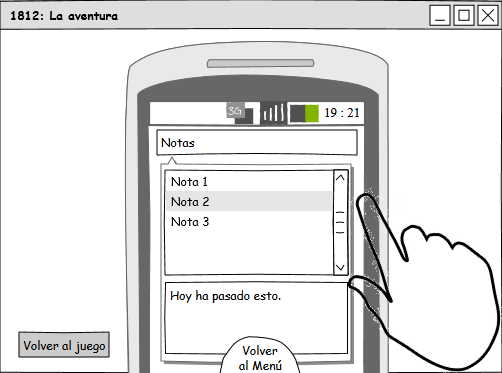
\includegraphics[scale=0.7]{notas.png}
            	\end{center}
            	\caption{Boceto de la pantalla de Notas}
            	\label{fig:notas}
            \end{figure}
            
            Lista y descripción de todos sus componentes:
            \begin{itemize}
            	\item \negrita{Lista de notas}: lista con las notas que relatan los sucesos importantes que han ocurrido en la partida hasta el momento. Se muestra el nombre de la nota, que suele es una frase corta resumiendo el suceso.
            	\item \negrita{Bloque de texto}: bloque de texto informativo más descriptivo sobre el suceso importante.
            	\item \negrita{Icono Volver al Menú}: al pulsarlo volvemos a la pantalla \emph{Menú Opciones}.
            	\item \negrita{Botón Volver al juego}: al pulsarlo volvemos a la pantalla de juego.
            \end{itemize}
            
            \newpage
            \subsection{Ajustes}
            A continuación el boceto de la pantalla \emph{Ajustes} :
            
            \begin{figure}[H] 
            	\begin{center}
            		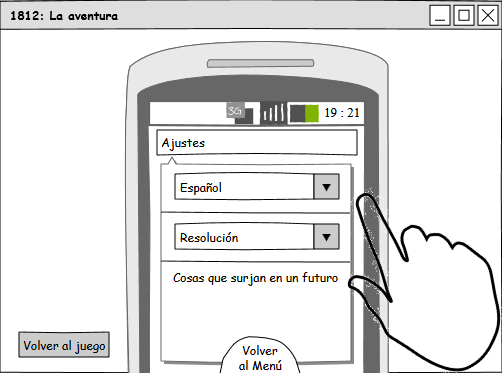
\includegraphics[scale=0.7]{ajustes.png}
            	\end{center}
            	\caption{Boceto de la pantalla de Ajustes}
            	\label{fig:ajustes}
            \end{figure}
            
            Lista y descripción de todos sus componentes:
            \begin{itemize}
            	\item \negrita{Lista despegable de idiomas}: lista despegable con los idiomas disponibles para el juego.
            	\item \negrita{Lista despegable de resolución}: lista despegable con las resoluciones de pantalla disponibles para el juego.
            	\item \negrita{Otros}: bloque destinado a futuros ajustes que puedan meterse en el videojuego.
            	\item \negrita{Icono Volver al Menú}: al pulsarlo volvemos a la pantalla \emph{Menú Opciones}.
            	\item \negrita{Botón Volver al juego}: al pulsarlo volvemos a la pantalla de juego.
            \end{itemize}
            
            %\newpage
            %\subsection{Salir}
        %\subsection{Trucos y \emph{Easter Eggs}}
        %Por ahora no hay intención de introducir trucos y \emph{Easter Eggs}.